%-*-coding: utf-8-*-
\chapter{Обзор предметной области}

\section{Описание проблемы}

Ошибки в коде программного обеспечения могут представлять большую
опасность и приводить с серьёзным убыткам. Например, в 2003-ем году
большое число компьютеров по всему миру было заражено вирусом SQL
Slammer~\cite{moore2003spread}, что приводило к отказу оборудования и
существенному замедлению трафика в сети Интернет в целом. Другим
примером служит червь Code-Red, убытки от которого оцениваются
миллиардами долларов~\cite{moore2002code}. Оба вируса использовали
уязвимости в программном коде, позволявшие осуществить выход за
пределы массива. Такие ошибки являются одними из наиболее опасных,
поскольку зачастую злоумышленик может, используя уязвимость, выполнить
произвольный код и/или получить права
суперпользователя~\cite{onesmashing}.

Наиболее актуальна данная проблема для языков C/C++. Дизайн этих
языков подразумевает высокую гибкость и производительность, жертвуя
безопасностью. Языки позволяют осуществлять произвольный доступ к
памяти и не имеют встроенных автоматических проверок корректности. Для
многих приложений данный недостаток является менее существенным, чем
производительность, поэтому языки C и C++ активно используются и по
сей день. Также порой выбор языка происходит по историческим
соображениям, когда приходится поддерживать старый код. Многие
операционные системы написаны на C/C++ из соображений гибкости и
производительности. Также существует большое число программ,
работающих с сетью и получающих данные извне, написанных на C/C++ из
соображений производительности. Уязвимости в таком программном
обеспечении являются крайне опасными, поскольку операционные системы
работают напрямую с аппаратными средствами, а ошибки в сетевых
приложениях могут быть эксплуатированы удалённо фактически любым
человеком.

В данной работе под выходом за пределы динамического массива
подразумевается обращение (чтение и запись) к памяти за пределами
выделенного участка памяти. Если существуют такие входные данные (то
есть любые данные, неизвестные заранее), что при запуске программы с
этими данными в ней присутствует инструкция, совершающая
выход за пределы массива, то такая инструкция считается ошибочной и
потенциально уязвимой. Задача состоит в поиске таких инструкций.

В связи с актуальностью проблемы ей уделено большое внимание учёных и
инженеров по всему миру. Известно большое число подходов к решению
данной задачи. Глобально их можно разделить на динамические и
статические.

Динамические подходы~\cite{cowan1998stackguard, ruwase2004practical,
  hastings1991purify} состоят в добавлении в программу дополнительных
проверок, предотвращающих обращение к памяти за пределами выделенного
буфера. Основное преимущество этого подхода в том, что он, как
правило, предотвращает большее число ошибок, поскольку значения всех
переменных известны в момент обращения к памяти. Однако такие подходы
существенно замедляют работу программы, что зачастую оказывается
неприемлимо в случаях, когда производительность стоит на первом
месте. Другим недостатком динамического подхода является тот факт, что
при наличии ошибки она будет обнаружена уже во время программы, что,
скорее всего, приведёт к остановке. Также динамические подходы
способны находить лишь ошибки, которые воспроизводятся на реально
выполняемых участках кода. На практике же нередко происходит так, что
какой-то фрагмент кода может не выполняться на протяжении очень
длительного времени, однако именно в нём может быть ошибка, которая
очень долго будет оставаться незамеченной.

Статический анализ, в отличие от динамического, производится без
запуска программы. Это позволяет исследовать все места в коде, даже
редко выполняемые, а также позволяет найти ошибки до реального
использования программы, пока они не проявили себя. Помимо этого
статический анализ никак не меняет исполняемый код, а значит, не
замедляет программу. В общем случае задача поиска всех выходов за
пределы массива в C/C++ без единого ложного срабатывания неразрешима
(это напрямую следует из проблемы
останова~\cite{turing1937computable}), поэтому одним из главных
недостатков статического анализа является необходимость ручного
рассмотрения результатов работы анализатора с целью выяснения, какие
из найденных ошибок действительно являются таковыми.

Таким образом, динамические и статические подходы имеют свои
преимущества и недостатки. В разных случаях имеет смысл применять
разные подходы (в том числе комбинацию подходов). Оба варианта
являются осмысленными и актуальными. В данной работе был сделан выбор
в пользу статического анализа. Поскольку задача неразрешима в общем
случае, требуется находить как можно больше ошибок в программах,
минимизируя при этом число ложных срабатываний. Важным требованием
является способность обрабатывать крупные программы, состоящие из
сотен тысяч строк, за разумное время. Как правило, приемлимым является
время порядка нескольких десятков минут. Это сопоставимо со временем
сборки проекта и позволяет, например, включить анализатор в систему
непрерывной интеграции.

Несмотря на огромное число исследований, посвящённых данной проблеме,
уязвимости, связанные с выходом за пределы массива продолжают
оставаться одними из наиболее часто встречаемых~\cite{uscert}. Таким
образом, на сегодняшний день задача не перестаёт быть
актуальной. Также стоит отметить, что большое число подходов,
описанных в статьях, находятся в закрытом доступе или же
поддерживаются на протяжении долгих лет. Большинство доступных
анализаторов решают более общую проблему поиска различных ошибок и
либо работают слишком долго на больших программах, либо находят
слишком мало ошибок, связанных с выходами за пределы массива.

\section{Обзор существующих решений}

Существует больше число статей, посвящённых статическому поиску
выходов за пределы динамического массива в C и C++. Отдельно стоит
отметить статью~\cite{shahriar2010classification}, в которой
представлена классификация различных подходов. В большинстве случаев
основной компромисс делается между скоростью работы, числом находимых
ошибок и точностью.

Наиболее простые анализаторы~\cite{viega2002token,flawfinder} не
учитывают поток управления и зависимости по данным в программе, а
выполняют лишь символьный анализ. Такие подходы просты в реализации и
работают очень быстро, однако точность анализа крайне низкая. По сути,
такие анализаторы лишь находят потенциально опасные места в программе
и эвристически сортируют их. В данной работе требуется большая
точность, поэтому необходимо учитывать семантику программы.

Некоторые подходы~\cite{larochelle2001statically, hackett2006modular,
  dor2003cssv} основаны на использовании пользовательских аннотаций
для вывода ограничений на значения переменных. В таком случае
разработчик пишет аннотации в различных местах в коде. Аннотации
сообщают анализатору различные инварианты, гарантированно
выполняющиеся в определённом месте. Например, что значение переменной
ограничено сверху определённым значением. Анализатор работает в
предположении, что все инварианты, задаваемые аннотациями, выполнены,
что ползволяет повысить точность анализа. Некоторые анализаторы также
проверяют корректность аннотаций. Недостатком таких подходов
является необходимость добавления аннотаций в код. В некоторых случаях
это не представляет большой проблемы, особенно если приложение пишется
с нуля. Однако для больших программ добавление аннотаций к каждой
функции может занять чрезвычайно много времени. Наибольшую трудность
представляет аннотирование старого кода, написанного незнакомыми
людьми. Поскольку основной целью работы является анализ крупных
программ, использование аннотаций не имеет большого смысла, и в этой
работе они не используются.

Также для решения рассматриваемой задачи можно использовать подходы,
базирующиеся на ограниченной проверке моделей (bounded model
checking)~\cite{cordeiro2012smt, merz2012llbmc}. Такой подход
позволяет проверять различные свойства программы, включая наличие
выходов за пределы массива. Для этого программа описывается системой
переходов, проверяемое свойство формулируется в виде логического
утверждения, после чего выполнимость условия проверяется SAT- или
SMT-решателем. При этом рассматриваются пути в программе с
ограниченной глубиной, чтобы гарантировать, что анализ
закончится. Такие подходы обладают хорошей точностью и позволяют
проверять различные свойства программы, однако это достигается за счёт
низкой производительности. Проблема заключается в экспоненциальном
росте сложности задачи при увеличении числа ветвлений в программе. В
результате такие подходы не могут быть применены к большим программам.

Подходы, описанные в статьях~\cite{wagner2000first,
  ganapathy2003buffer, larochelle2001statically}, в целом весьма
похожи. Сначала анализатор обходит весь код программы и строит систему
ограничений на значения переменных. Затем система решается с
использованием различных алгоритмов (зависит от анализатора). В
результате выводится как можно более точная оценка возможных значений
переменных. После этого обращения к массиву анализируются, исходя из
выведенных ограничений. Подходы различаются в основном
чувствительностью анализа (учётом контекста, наличием межпроцедурного
анализа и т. д.), гранулярностью анализа и способом разрешения
ограничений. За счёт различных эвристик такие подходы работают
относительно быстро на программах среднего размера, однако на больших
программах получается слишком много ограничений, и их решение занимает
слишком много времени.

В статье~\cite{xie2003archer} описан подход, способный обрабатывать
программы, состоящие из сотен тысяч строк кода. Этот подход использует
полностью символьный анализ, в рамках которого возможные значения
переменных представлены символьно, что позволяет учитывать зависимости
между переменными, не зная конкретных значений. Анализ является
межпроцедурным, что существенно повышает точность на практике. При
анализе конкретной функции происходит проход по графу потока
управления всей функции. Каждая инструкция может модифицировать
контекст анализатора. При обработке условных переходов выполняется
проверка значения, влияющего на переход. Если значение не может быть
посчитано статически, происходит размножение контекста, и анализатор
продолжает работу с большим числом контекстов. При обработке обращения
к массиву анализатор может непосредственно вывести, возможно ли
переполнение. За счёт отсутствия необходимости разрешать системы
ограничений такой подход работает быстрее предыдущих.

Более современная идея заключается в использовании анализа «по
требованию», при котором анализируются только те инструкции программы,
которые влияют на результат какого-то запроса. Например,
статья~\cite{le2008marple} использует анализ по требованию для поиска
выходов за пределы массива. Основная цель данной идеи заключается в
уменьшении числа анализируемых путей программы и, следовательно,
повышении скорости анализа. «Требование» анализа возникает в местах,
где может выполниться какой-то запрос (в данном случае в местах
обращения к массиву). Затем происходит распространение запроса в
обратном направлении по графу потока управления. В процессе
распространения происходит сбор информации о значениях переменных,
влияющих на запрос. Обход заканчивается, когда ответ на запрос может
быть однозначно вычислен или при достижении входа в функцию. На
практике такой подход работает существенно быстрее аналогичных
подходов, анализирующих программу целиком. Схожие идеи применены также
в статьях~\cite{ding2012detection, ding2014abor, li2010practical}.

\section{Обзор статьи~\cite{li2010practical}}

На основании проведённого изучения литературы было принято решение
использовать алгоритм, описанный в статье \cite{li2010practical}, в
качестве базового. Во-первых, этот подход является легковесным, что
позволяет достаточно быстро обрабатывать большие программы. Во-вторых,
результаты, представленные в статье, говорят о том, что анализатор
способен находить много ошибок в крупных открытых проектах. В-третьих,
несмотря на довольно хорошие результаты, авторы также отмечают наличие
ложных срабатываний и спорных ситуаций, в которых алгоритм не может
принять однозначное решение. А значит, у этого подхода есть
пространство для улучшений.

\subsection{Static Single Assignment}

Описанный в статье алгоритм рассматривает программу, представленную в
Static Single Assignment форме~\cite{cytron1991efficiently} (SSA). Такое
представление является весьма удобным для статического анализа. SSA
форма имеет две особенности. Во-первых, значение любой переменной
присваивается ровно один раз. Во-вторых, вводится специальная
инструкция $\phi$, возвращающая один из своих аргументов в зависимости
от того, из какого предка поток управления пришёл в эту инструкцию. За
счёт этого удаётся представить различные языковые конструкции, при
которых происходит изменение значения переменной, например, циклы.

\begin{figure}
    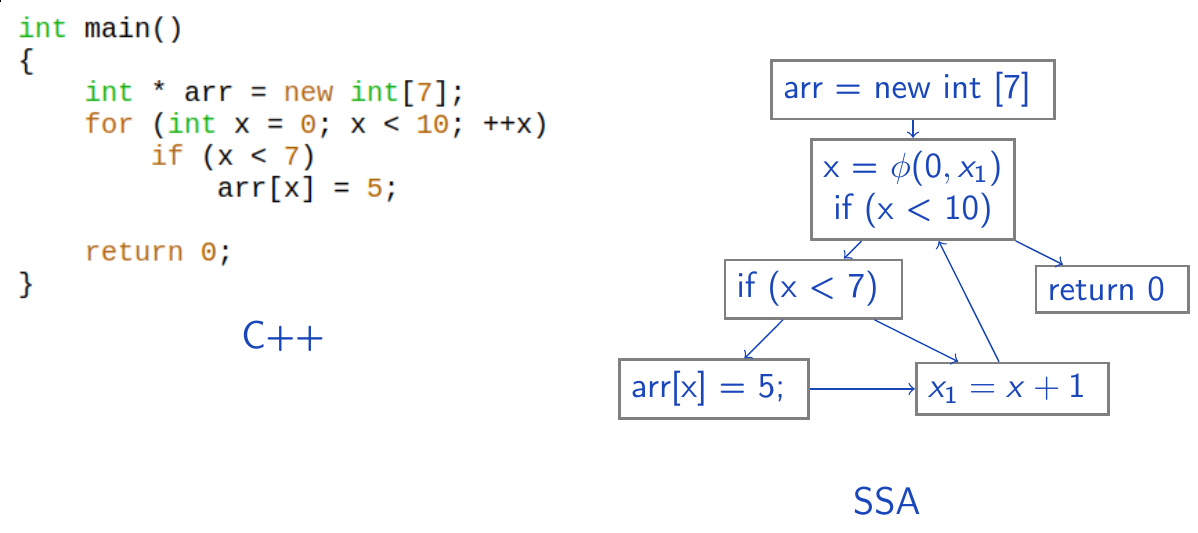
\includegraphics[width=\textwidth]{ssa.png}
    \caption{SSA форма}
    \label{fig:ssa}
\end{figure}

На рисунке~\ref{fig:ssa} представлен пример SSA формы. В C++ программе
значение переменной $x$ меняется на каждой итерации цикла. Однако в
SSA форме значение переменной может присваиваться только один раз. Для
этого значение $x$ определяется как $\phi$ от начального значения
($0$) и дополнительной переменной $x_1$, определённой как $x +
1$. Таким образом, на каждой итерации цикла значение переменной $x$
будет на 1 больше предыдущего, что соответствует C++ коду.

\subsection{Символьные вычисления}

Алгоритм базируется на символьных вычислениях для обнаружения выходов
за пределы массива. Символьные вычисления позволяют учесть зависимости
между переменными, не зная их численных значений. В основе алгоритма
лежит понятие символьного выражения (symbolic expression), а также
символьного диапазона (symbolic range).

Символьным выражением может быть число, переменная, афинная функция
другого символьного выражения, а также два специальных значения $\bot$
и $\top$, соответствующих наименьшему и наибольшему возможному
значению. Для символьных выражений естественным образом определяются
операции сложения, вычитания, умножения и деления. Также вводится
частичный порядок ($\prec$) следующим образом: $E_1 \prec E_2$ тогда и
только тогда, когда $E_1 - E_2$ не больше нуля (для всех непостоянных
значений).

Символьный диапазон определяется как пара символьных выражений. Для
символьных диапазонов также определяются операции сложения, вычитания,
умножения и деления. К ним добавляются операции пересечения и
объединения. Для переменной $V$ вводится понятие define range $S_V$
--- символьного отрезка, соответствующего диапазону возможных значений
$V$ в месте её определения. Так как программа представлена в SSA
форме, определение переменной и присвоение ей значения происходит
ровно в одном месте. Также вводится понятие use range для переменной
$V$ и инструкции $P$: $S_{V,P}$. Этот символьный диапазон
соответствует возможным значениям $V$ в месте инструкции $P$. Такой
диапазон может отличаться от define range, поскольку на пути к
инструкции $P$ могут быть условные переходы с предикатами,
ограничивающими значение $P$.

\subsection{Вычисление диапазонов}

Для расчёта описанных выше диапазонов рассматриваются два вида
зависимостей: зависимости по данным и зависимости потока управления.

Зависимости по данным используются для расчёта define range $S_V$, то
есть диапазона возможных значений $V$ в месте определения. Он
вычисляется через use range аргументов в инструкции, определяющей
$V$. Например, если $V = a + b$, то $S_V = S_{a, V} + S_{b, V}$. Для
$V = \phi(a, b)$ используется объединение, поскольку $\phi$ может
вернуть любой из аргументов: $S_V = S_{a, V} \cup S_{b, V}$. Аналогично
вычисляется define range для других инструкций.

Зависимости потока управления используются для уточнения диапазона
значений переменной $V$ в инструкции $P$ ($S_{V, P}$), который может
отличаться от $S_V$. Для уточнения используются условные переходы,
лежащие на путях $P$, в которых используются предикаты, затрагивающие
$V$. При этом рассматриваются только условные переходы,
удовлетворяющие двум условиям. Во-первых, узел, соответствующий $P$ в
графе потока управления, должен доминироваться узлом, соответствующим
условному переходу. Другими словами, любой путь из входа в функцию в
инструкцию $P$ должен проходить через рассматриваемый условный
переход. Во-вторых, $P$ должна быть достижима только из одного потока
условного перехода. В таком случае условие, соответствующее этому
потомку, считается выполненым, и применяется для уточнения диапазона
значений $V$. Например, для условия $V \geq y$ диапазон значений $V$
будет пересечён с $[y, \top]$. Также учитываются предикаты, в которых
$V$ фигурирует не напрямую, а через афинное преобразование. Например,
$2 * V + 3 < W$. В этом случае диапазон будет пересечён с $[\bot,
\frac{W - 3}{2}]$.

Выход за пределы массива размера $n$ при обращении по индексу $index$
(инструкция $P$) фиксируется, если
$S_{n, P}^{max} \prec S_{index, P}^{max}$, то есть максимальная оценка
размера меньше либо равна максимальной оценки индекса, или $S_{index, P}^{min} \prec
-1$, то есть индекс может быть отрицательным. Если $S_{index, P}^{max}
\prec S_{n, P}^{min} - 1$ и $0 \prec S_{V, P}^{min}$, то выход за
пределы массива точно не может случиться. В остальных случаях алгоритм
не может однозначно определить, возможно ли переполнение. В таких
случаях алгоритм не сообщает об ошибке, поскольку это приводило бы к
слишком большому числу ложных срабатываний, и анализатором было бы
очень сложно пользоваться.

Алгоритм использует идею анализа «по требованию». Вычисление
диапазонов значений начинается в инструкциях, в которых происходит
непосредственное обращение к массиву. Для проверки корректности
вычисляются диапазоны значений размера массива и индекса, по которому
производится обращение. Поскольку в графе зависимостей между
переменными могут присутствовать циклы, используется специальный
итерационный алгоритм, гарантирующий прогресс и итоговое завершение
работы анализатора (итерации выполняются до достижения неподвижной
точки).

\chapterconclusion

В данной главе была подробно описана проблема выхода за пределы
динамического массива в C/C++ программах, показана её
актуальность. Был приведён обзор существующих решений этой проблемы,
описаны ключевые характеристики различных статических
подходов. Наиболее оптимальными, с точки зрения производительности,
являются подходы, использующие анализ «по требованию». Также был обоснован
выбор алгоритма из статьи~\cite{li2010practical} в качестве базового
подхода для данной работы, приведён более подробный обзор этого
алгоритма.

\FloatBarrier
